\section{Scaling Experiments}

\subsection{Experimental Setup}

\paragraph{Hyperparameters.}
Following the $\boldsymbol{\mu}$P protocol, we perform a learning rate sweep on the 1.7B model with AdamW between [$10^{-3}$, $10^{-2}$] and find $5 \times 10^{-3}$ to be the optimal value.
Training uses 500 warmup steps, a global batch size of $\sim$4M tokens (1024 sequences $\times$ 4096 tokens each), and a cosine learning rate decay reduced to $10\%$ peak. We use BF16 mixed-precision training.

Following Kimi Moonlight~\citep{liu2025muonscalablellmtraining}, all optimizers use a weight decay of 0.1. However, distinct from their approach of aligning updates to AdamW RMS (intended to reuse current scaling laws), we find that spectral $\boldsymbol{\mu}$P LR scaler outperforms the uniform 0.2 update-rms alignment (\cref{sec:lr_scaler}).
For msign coefficients, we use the Polar Express method~\citep{amsel2025polarexpressoptimalmatrix} with 8 Newton–Schulz iterations\footnote{We tested 5 and 8 iterations as well as different msign coefficients and observed negligible differences in training loss (< 1e-3). We retain 8 iterations for improved numerical accuracy.}.
We employ Nesterov momentum and, by default, split attention heads and FFN gate/up projections for separate initialization and optimization. For Spectral Sphere, we set the $\lambda$-solver's maximum iterations to 20, Lagrange solver precision tolerance to 2e-4, and remove weight decay for all hidden 2D weights, as retraction maintains the weight constraint (\cref{sec:retraction}).

\paragraph{Training Data.}
We use the OLMo-Mix-1124 dataset~\citep{olmo20252olmo2furious}, tokenized with the OLMo-2 tokenizer. We randomly sample 100 billion tokens for training and reserve 1 billion tokens for validation. Data indices are built offline to guarantee a deterministic training order.

\paragraph{Benchmarks.}
We primarily evaluate on the following downstream tasks: ARC~\citep{clark2018arc}, BoolQ~\citep{clark2019boolq}, CSQA~\citep{talmor2019csqa}, HellaSwag~\citep{zellers2019hellaswag}, PIQA~\citep{bisk2020piqa}, WinoGrande~\citep{sakaguchi2021winogrande} and LAMBADA~\citep{paperno2016lambada}.


\subsection{Dense 1.7B}
\label{subsec:dense_1.7b}

We adopt the architecture configuration of Qwen3-1.7B~\citep{yang2025qwen3technicalreport}, replacing its original tokenizer with that of OLMo-2~\citep{olmo20252olmo2furious}. The core architecture utilizes Grouped Query Attention (GQA), QK-Norm, SwiGLU activations, Rotary Positional Embeddings (RoPE), and pre-normalization RMSNorm. We do not tie the embedding and the head.


\begin{figure}[ht]
    \centering
    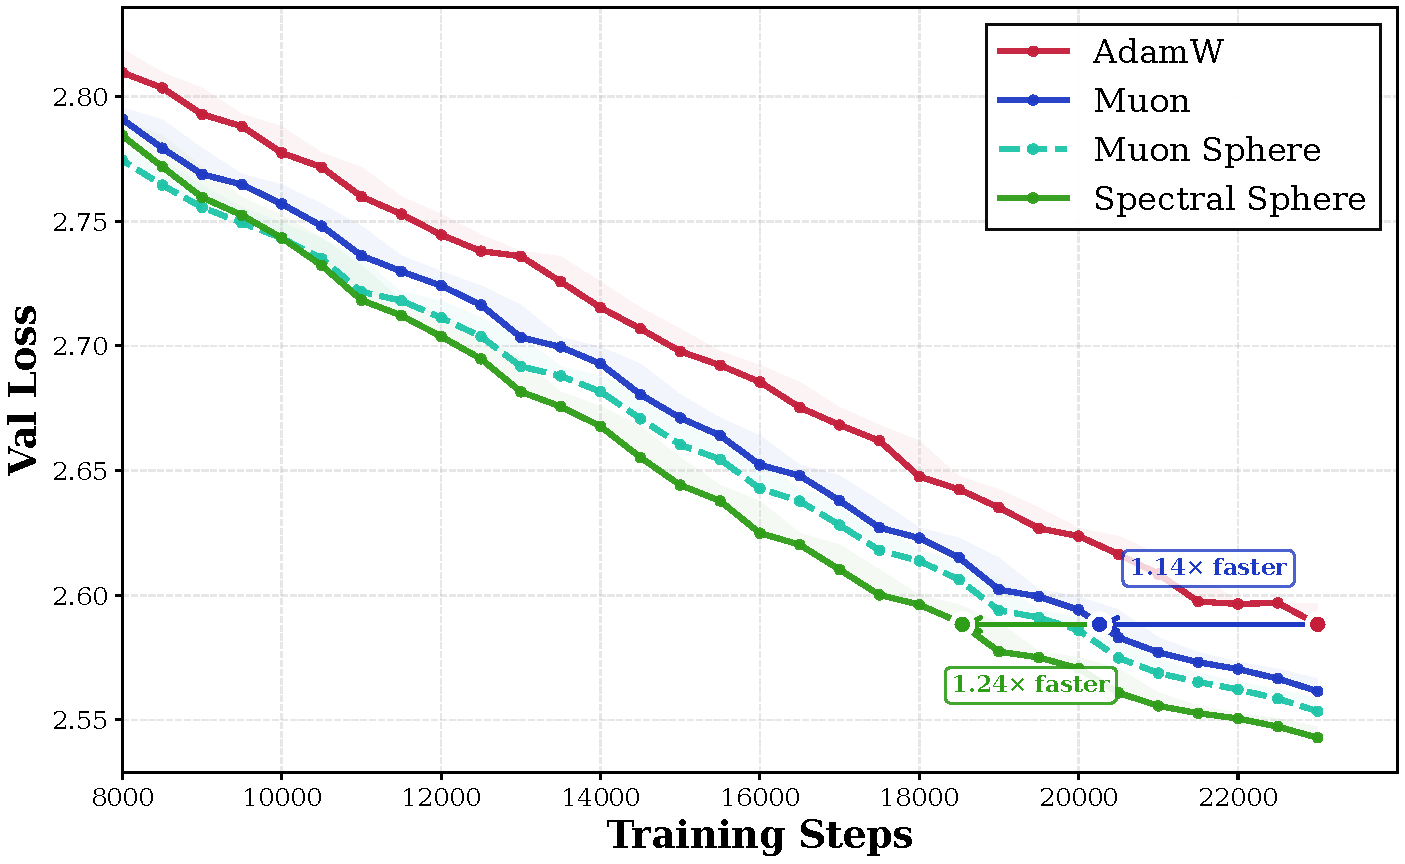
\includegraphics[width=0.5\linewidth]{figures/exp/dense_val_loss_comparison.pdf}
    \caption{
    \textbf{Validation loss of training dense 1.7B model on 100B tokens.}
    As a reference point, \textcolor{AdamWColor}{AdamW} attains a final validation loss of 2.588 at 23k steps. The overall setup favors \textcolor{AdamWColor}{AdamW}, since the learning rate is set for it (5e-3), rather than the higher optimal rate (1e-2) for \textcolor{MuonColor}{Muon} and \textcolor{SpectralSphereColor}{Spectral Sphere}. Even under this setting, spectral-based optimizers exhibit higher efficiency: \textcolor{MuonColor}{Muon} reaches the same validation loss level in 12\% fewer steps, while \textcolor{SpectralSphereColor}{Spectral Sphere} does so in 19\% fewer steps.
    }
    \label{fig:qwe3_1.7B_dense}
\end{figure}



\begin{table}[ht]
\centering
\caption{Performance comparison of different optimizers on Dense 1.7B models.}
\label{tab:commonsense_results}
\resizebox{\linewidth}{!}{
\begin{tabular}{l|c|cccccccc|c}
\toprule
\multirow{2}{*}{\textbf{Optimizer}}    & \textbf{LMB.} & \textbf{LMB.} & \textbf{CSQA} & \textbf{PIQA} &    \textbf{Hella.} & \textbf{Wino.} & \textbf{ARC-e} &  \textbf{ARC-c}  & \textbf{BoolQ} &  \textbf{Avg.} \\
 &  (PPL) $\downarrow$ &  (Acc) $\uparrow$  & (Acc) $\uparrow$ &   (Acc) $\uparrow$  & (Acc) $\uparrow$  & (Acc) $\uparrow$ & (Acc) $\uparrow$ & (Acc) $\uparrow$ & (Acc) $\uparrow$ & (Acc) $\uparrow$ \\
\midrule
\textcolor{AdamWColor}{AdamW} & 5.40 & 63.71 & 19.66 & 74.70 & 47.90 & 62.59 & 68.81 & 37.37 & 63.24 & 54.75\\
\textcolor{MuonColor}{Muon}   & 5.05 & 65.19 & 19.00 & 75.35 & 48.91 & 61.72 & 70.24 & 37.46 & 64.22 & 55.26\\
\textcolor{MuonSphereColor}{MuonSphere}  & \textbf{4.87} & \textbf{65.55} & 20.07 & 74.97 & 49.20 & 62.83 & 71.51 & \textbf{38.40} & \textbf{66.97} & 56.19\\
\textcolor{SpectralSphereColor}{Spectral Sphere} & 5.00 & 65.07 & \textbf{21.05} & \textbf{75.95} & \textbf{49.25} & \textbf{63.77} & \textbf{71.80} & 38.31 & 65.57 & \textbf{56.35} \\
\bottomrule
\end{tabular}
}
\end{table}


\subsection{MoE 8B-A1B}

The configuration largely follows DeepSeek-V3~\citep{deepseekai2025deepseekv3technicalreport}. The model has 27 layers: the first is a standard dense FFN, followed by 26 MoE layers. We utilize 64 experts in total, with a top-4 routing expert plus 1 shared expert.

\textbf{Router and Load Balancing.} The router is implemented in FP32 precision. We adopt the auxiliary-loss-free strategy~\citep{wang2024auxiliarylossfreeloadbalancingstrategy}, which demonstrated superior expert load balancing compared to global auxiliary loss~\citep{qiu2025demonsdetailimplementingload} in our ablations. We enable expert bias with an update rate of 0.001. The sequence-level auxiliary loss is removed, as we find it redundant when expert bias is enabled. we use a sigmoid gate with top-$k$ scores renormalized and scaled by 2. (see~\cref{app:moe_scaling}). To evaluate router load balancing, we employ Maximal Violation (MaxVio)~\citep{wang2024auxiliarylossfreeloadbalancingstrategy}, where $0$ indicates perfect balance. As
shown in~\cref{fig:moe_8b_a_1b_maxvio_valloss}, weight spectral normalization
effectively promotes balanced routing, leading to superior validation loss.
\begin{figure}[ht]
    \centering
    \begin{subfigure}{0.48\linewidth}
        \centering
        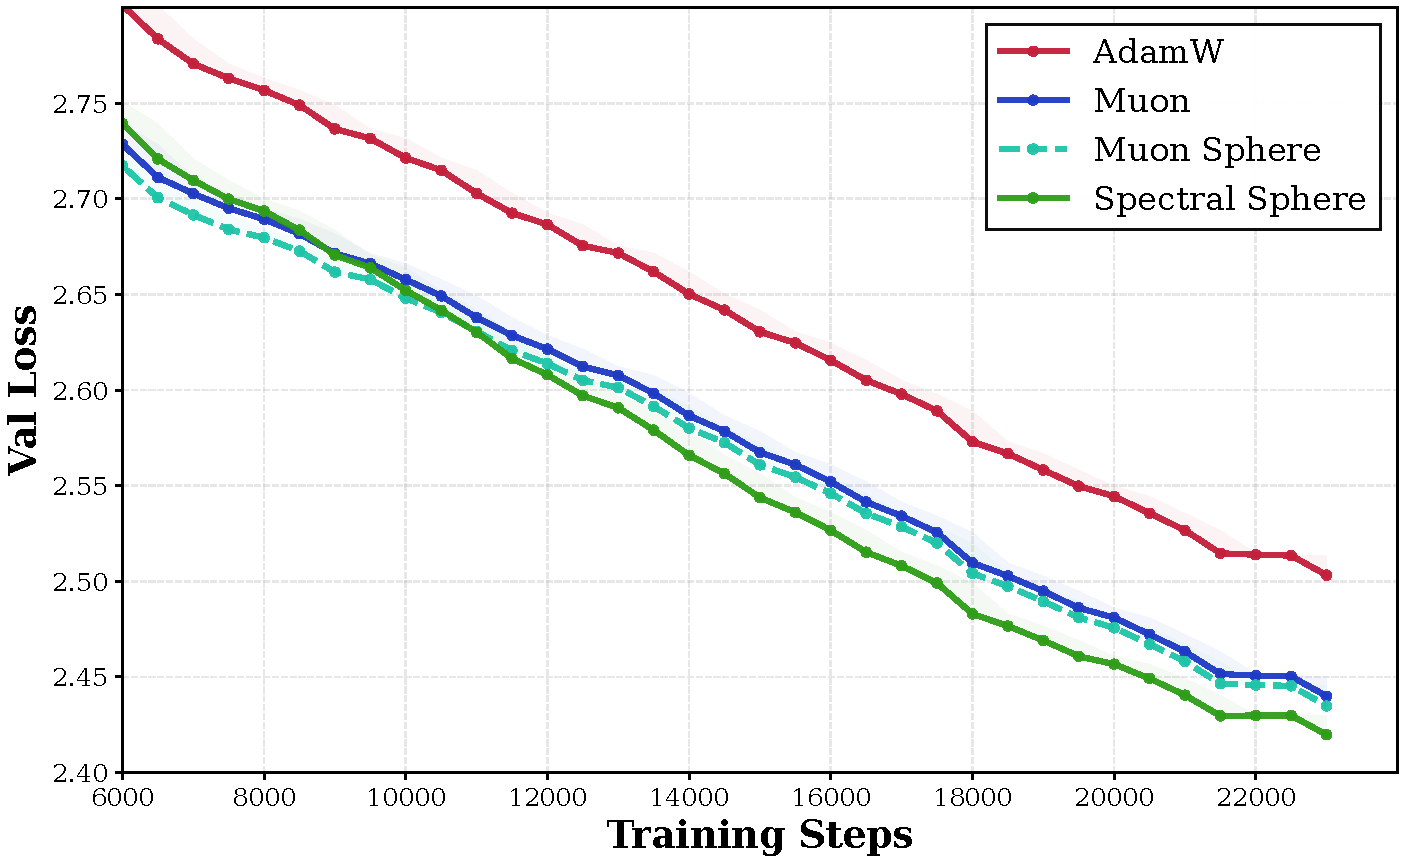
\includegraphics[width=\linewidth]{figures/exp/moe_val_loss_comparison}
        \caption{Validation Loss across four optimizers.}
    \end{subfigure}
    \hfill
    \begin{subfigure}{0.48\linewidth}
        \centering
        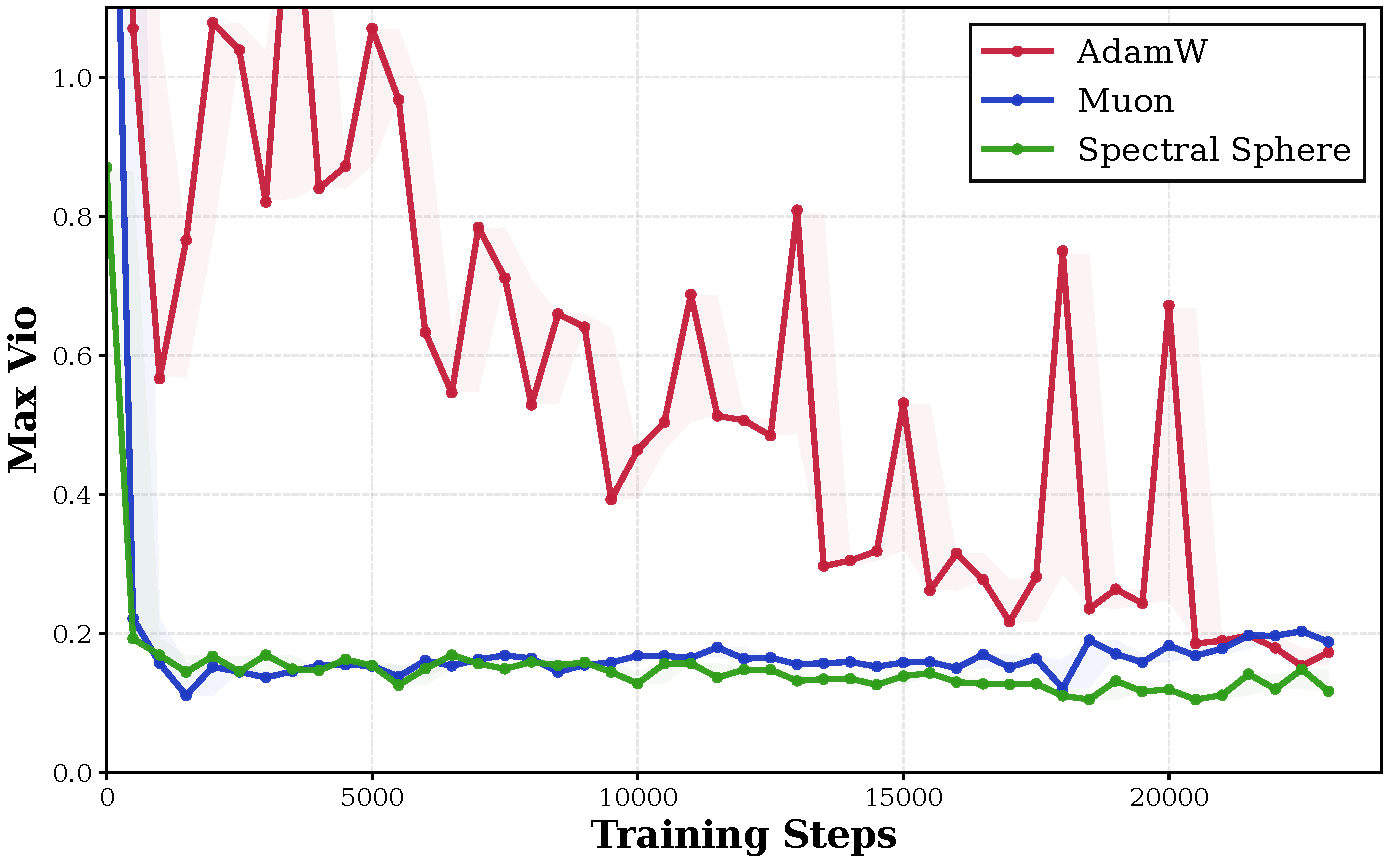
\includegraphics[width=\linewidth]{figures/exp/max_vio_comparison}
        \caption{MaxVio as a MoE load-balance metric.}
    \end{subfigure}
    \caption{\textbf{MoE 8B-A1B training.} \textcolor{SpectralSphereColor}{Spectral Sphere} achieves the lowest validation loss while maintaining the best expert load balance. In contrast, \textcolor{AdamWColor}{AdamW} exhibits substantially larger MaxVio with frequent spikes, indicating unstable routing and poorer utilization of effective model capacity. Compared to \textcolor{MuonColor}{Muon}, constraining each expert on the spectral sphere further improves load balance.}
    \label{fig:moe_8b_a_1b_maxvio_valloss}
\end{figure}

\subsection{DeepNet 200-Layer}
To evaluate the stability of different optimizers under extreme depth, we extended the baseline's 28 layers to 200 layers. This deep and narrow serves as a stress test for stability. The training loss in~\cref{fig:deepnet} shows that Spectral Sphere outperforms baselines with lower loss and higher stability.
\begin{figure}[ht]
    \centering
    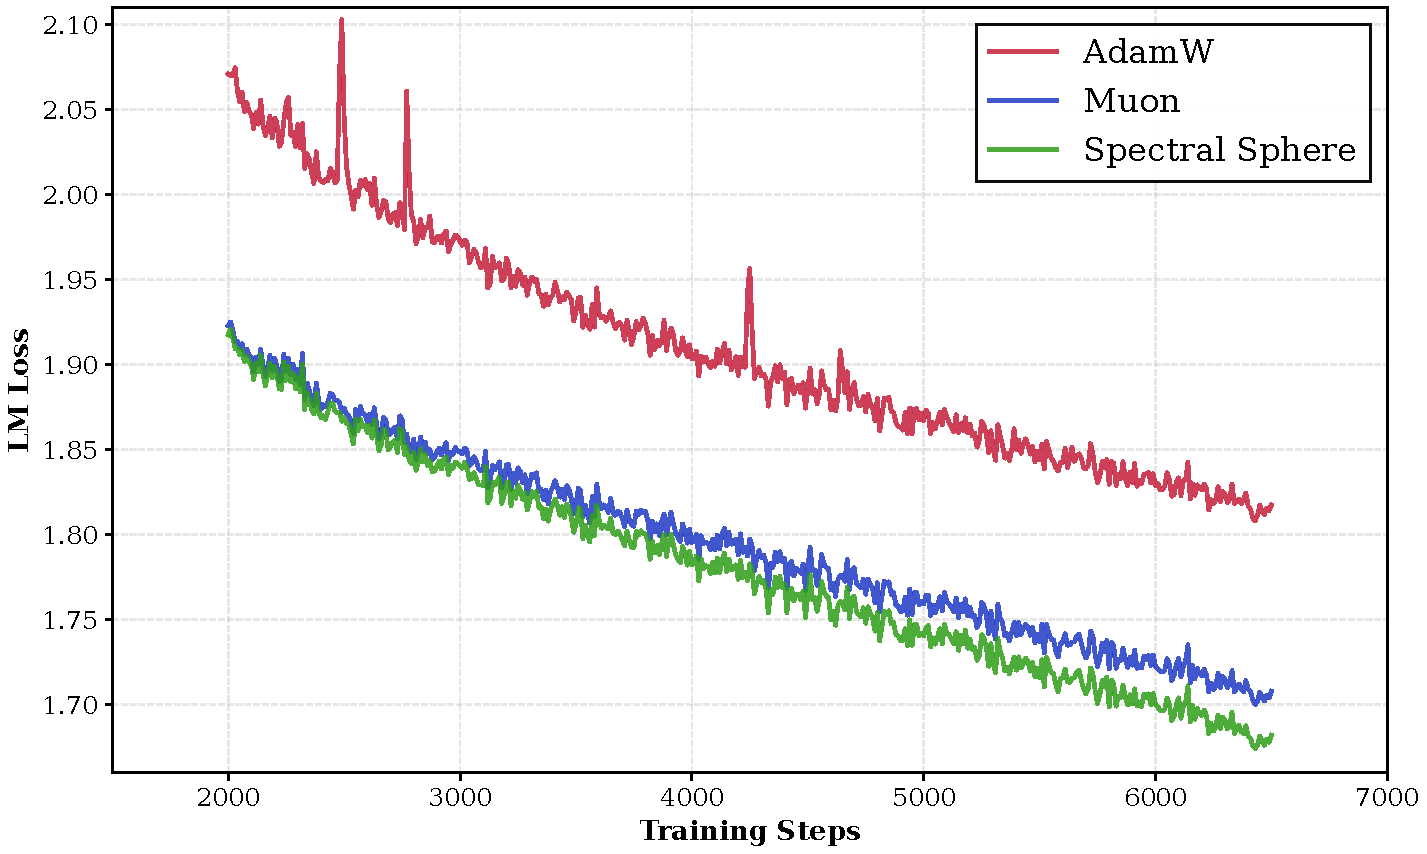
\includegraphics[width=0.5\linewidth]{figures/exp/deepnet_train_loss.pdf}
    \caption{\textbf{Deepnet 200 layers training loss.} \textcolor{AdamWColor}{AdamW} shows pronounced instability, characterized by frequent loss spikes and a growing gap in performance relative to spectral-based optimizers. \textcolor{SpectralSphereColor}{Spectral Sphere} attains both the lowest loss and the highest stability.}
    \label{fig:deepnet}
\end{figure}
